\documentclass{standalone}
\usepackage{tikz}

\begin{document}
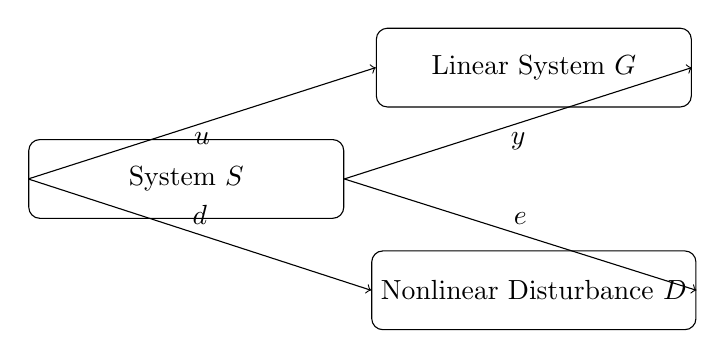
\begin{tikzpicture}[node distance=2cm]
    % Define styles for nodes and arrows
    \tikzstyle{box} = [rectangle, draw=black, fill=white, text centered, rounded corners, minimum width=4cm, minimum height=1cm]
    
    % Nodes
    \node (S) [box] {System $S$};
    \node (G) [box, above right of=S, xshift=3cm] {Linear System $G$};
    \node (D) [box, below right of=S, xshift=3cm] {Nonlinear Disturbance $D$};
    
    % Arrows
    \draw[->] (S.west) -- node[midway, below] {$u$} (G.west);
    \draw[->] (S.east) -- node[midway, below] {$y$} (G.east);
    \draw[->] (S.west) -- node[midway, above] {$d$} (D.west);
    \draw[->] (S.east) -- node[midway, above] {$e$} (D.east);
\end{tikzpicture}
\end{document}